\documentclass{beamer}
\usepackage{amsfonts,amsmath,oldgerm}
\usepackage[utf8]{inputenc}
\usepackage{hyperref}
\usepackage[portuguese, brazil, english]{babel}
\usepackage{minted}
\usetheme{sintef}
\usepackage[ddmmyyyy]{datetime}
\hypersetup{
	colorlinks=true,
	linkcolor=white,
	filecolor=blue,      
	urlcolor=blue,
	pdftitle={Aprendendo a Programar em Python - Módulo 01}
}
\newcommand{\testcolor}[1]{\colorbox{#1}{\textcolor{#1}{test}}~\texttt{#1}}

\usefonttheme[onlymath]{serif}

\titlebackground*{assets/background}

\newcommand{\hrefcol}[2]{\textcolor{cyan}{\href{#1}{#2}}}

\title{Introdução ao Python}
\subtitle{Aprendendo a Programar com Python}
\course{Módulo 01}
\author{\href{mailto:augusto.mathias@sesp.pr.gov.br}{Augusto Mathias Adams}}

\begin{document}
\maketitle
\footlinecolor{maincolor}

\begin{frame}

O Nivelamento de \textbf{\textit{Conceitos de Programação - Introdução ao Python }}tem como objetivo introduzir os participantes à linguagem de programação \textit{Python}, fornecendo as habilidades básicas para escrever programas funcionais, compreender conceitos fundamentais e promover a resolução de problemas. Ao final do nivelamento, os alunos estarão preparados para aplicar seus conhecimentos em projetos pessoais ou profissionais.

\end{frame}

\section{Ementa}

\begin{frame}{Pré-requisitos}
	Requisitos mínimos:
	\begin{itemize}
		\item Nenhum conhecimento prévio de programação é necessário.
		\item Um computador com \textbf{\textit{Python}} instalado.
	\end{itemize}
	É desejável:
	\begin{itemize}
		\item \textit{git} instalado (para baixar os exercicios)
		\item Conhecimentos mínimos de \textit{Docker} (será ministrado ao longo do curso)
	\end{itemize}
\end{frame}



\begin{frame}{Conteúdo do Nivelamento}
	O conteúdo deste nivelamento será dividido em 5 partes:
	\begin{itemize}
		\item \textbf{\textit{Módulo 1: }} introdução ao \textit{Python} e princípios básicos de algoritmos.
		\item \textbf{\textit{Módulo 2: }} introdução ao uso de pacotes e programação procedural com \textit{Python} e introdução ao pacote \textit{camera-discovery}.
		\item \textbf{\textit{Módulo 3: }} introdução à programação orientada a objetos e conceitos de banco de dados.
		\item \textbf{\textit{Módulo 4: }} introdução ao \textit{Django} - \textit{Framework} de desenvolvimento web usando python.
		\item \textbf{\textit{Módulo 5: }} produção de um sistema de monitoramento de câmeras usando os pacotes \textit{camera-discovery} e \textit{Django}.
	\end{itemize}
\end{frame}

\begin{frame}{Conteúdo do Nivelamento}
	Ao final de cada módulo, será proposta uma lista de exercícios de fixação do conteúdo visto em sala de aula.
\end{frame}

\begin{frame}{Conteúdo do Nivelamento}
	Bibliografia:
	\begin{itemize}
		\item \href{bibliografia/Beginning Programming with Python for Dummies.pdf}{\textbf{\textit{Beginning Programming with Python for Dummies}}}
		\item \href{bibliografia/Algorithms For Dummies.pdf}{\textbf{\textit{Algorithms for Dummies}}}
		\item \href{bibliografia/django-for-beginners-build-websites-with-python-amp-django_compress.pdf}{\textbf{\textit{Django for Beginners}}}
		\item \href{https://django-book.readthedocs.io/en/latest/}{\textbf{\textit{Django Book}}}
		\item \href{https://books.agiliq.com/projects/django-orm-cookbook/en/latest/}{\textbf{\textit{Django ORM Cookbook}}}
		\item \href{bibliografia/The Definitive Guide to Django - Apress.pdf}{\textbf{\textit{The Definitive Guide to Django}}}
		\item \href{bibliografia/Apostila_Modulo_01.pdf}{\textbf{\textit{Apostila Módulo 01}}}
	\end{itemize}
\end{frame}

\section{Introdução ao Python}
\subsection{Ementa}
\footlinecolor{maincolor}
\begin{frame}{Objetivos do Módulo}
\begin{itemize}
	\item Do que se trata \textbf{\textit{programar}}.
	\item O que significa o termo \textbf{\textit{algoritmo}}.
	\item Onde encontrar informações sobre como instalar o \textbf{\textit{Python}}.
	\item \textbf{\textit{Sintaxe e Estrutura de Dados}}.
	\item \textbf{\textit{Funções em Python}}.
	\item Primeira Aplicação em \textbf{\textit{Python}}.
	\item Comentários na sua primeira aplicação.
\end{itemize}
\end{frame}

\subsection{Conceitos De Programação}

\begin{frame}{Conceitos de Programação}

	Programar é:
	
	\begin{itemize}
		\item Ato de escrever um conjunto de instruções ou algoritmos que um computador pode executar para realizar uma tarefa específica.
		\item Criação de código em uma linguagem de programação que segue uma sintaxe e estrutura definidas.
		\item Requer habilidades lógicas e analíticas para que as instruções sejam escritas de forma clara e precisa.
	\end{itemize}

\end{frame}

\begin{frame}{Conceitos de Programação}
	
	Programar não é:
	
	\begin{itemize}
		\item Falta de planejamento e análise antes de começar a escrever o código.
		\item Ausência de comentários explicativos.
		\item Uso excessivo de linhas de código redundantes ou desnecessária.
		\item Mistura de diferentes estilos e convenções de codificação.
		\item Dificuldade em manter e fazer modificações no código devido à falta de estrutura.
	\end{itemize}
	
\end{frame}

\subsection{Algoritmos}

\begin{frame}{Algoritmo}
	
	Definições:
	
	\begin{itemize}
		\item \textbf{\textit{Algoritmo:}} sequência de passos usada para resolver um problema, fornecendo uma solução específica.
		\item Para ser considerado algoritmo:
		\begin{itemize}
			\item \textbf{\textit{Finito}}: eventualmente resolve o problema. 
			\item \textbf{\textit{Bem definido: }} série de passos precisa e etapas compreensíveis. 
			\item \textbf{\textit{Efetivo: }} resolve todos os casos do problema para o qual foi definido. 
		\end{itemize}
	\end{itemize}
	\alert{\textbf{\textit{Lembre-se:}}} \textbf{\textit{seguindo os passos da receita, conseguimos fazer o bolo!}}
\end{frame}

\begin{frame}{Algoritmos}
\begin{columns}
	\begin{column}{0.5\textwidth}
		\centering
		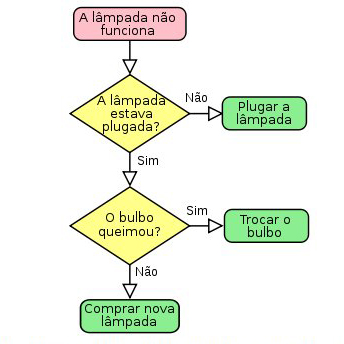
\includegraphics[width=0.7\textwidth]{imagens/fluxograma-exemplo.jpg}
	\end{column}
	\begin{column}{0.5\textwidth}
		\centering
		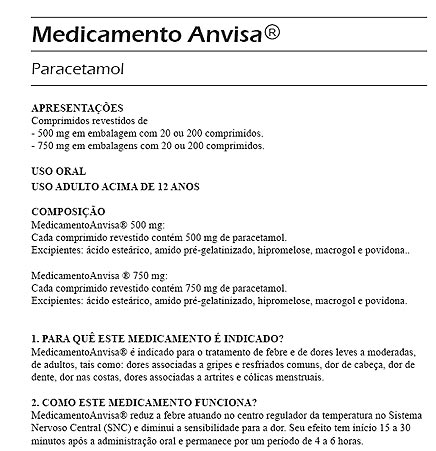
\includegraphics[width=0.7\textwidth]{imagens/nao_e_algoritmo.jpg}
	\end{column}
\end{columns}
\end{frame}

\begin{frame}{Algoritmos}
	Algoritmos comuns (implementados na maioria das linguagens):
	\begin{itemize}
		\item Algoritmos de Busca
		\item Algoritmos de Classificação e Ordenação
		\item Algoritmos de Transformação de Dados
		\item Algoritmos de Agendamento
		\item Algoritmos de Criptografia
		\item Geração de números pseudo-aleatórios
	\end{itemize}
\end{frame}

\section{Linguagem Python}

\subsection{O que é \textit{Python}}

\begin{frame}{O que é \textit{Python}}
	Do que se trata?
	\begin{itemize}
		\item \textbf{\textit{Definição:}} Linguagem de programação simples e versátil
		\item \textbf{\textit{Características:}}
		\begin{itemize}
			\item Multiplataforma
			\item Multiparadigma
			\item Linguagem Interpretada
		\end{itemize}
	\end{itemize}
\end{frame}

\begin{frame}{O que é \textit{Python}}
	Não posso gerar executável a partir do \textbf{\textit{Python}}? Pode.....
	\begin{itemize}
		\item Py2Exe
		\item PyInstaller
	\end{itemize}
\end{frame}

\begin{frame}{Instalando o \textit{Python}}
	Guia passo a passo para a instalação do \textbf{\textit{Python}}
	
	\begin{itemize}
		\item \href{bibliografia/Guia_Instalacao_Python.pdf}{\textbf{\textit{Apostila de Instalação}}}
	\end{itemize}
	
\end{frame}


\subsection{Sintaxe}

\begin{frame}{Estrutura e Sintaxe}
	
	A sintaxe do \textit{Python} é a forma como o código em \textit{Python} é escrito e
    estruturado. 
    
    \begin{itemize}
    	\item O código escrito em \textit{Python} é estruturado em blocos;
    	\item identação faz parte da estrutura;
    	\item sem necessidade de caracteres de abertura e fechamento de Blocos;
    	\item sem necessidade de terminador de linha;
    	\item comentários simples e multilinha;
    	\item Variáveis são utilizadas para armazenar valores e sua atribuição é feita através de um sinal de igualdade.
    \end{itemize}
	
\end{frame}

\begin{frame}[fragile]{Programa Simples Escrito em Python}
	Exemplo:
	\rule{\textwidth}{1pt}
	\scriptsize
	\begin{minted}{python}
		# comentário de uma linha
		# atribuindo o valor 5 a uma variável x
		x = 5
		if x > 5: 
			# inicio de um bloco
			print("x é maior que 5")
			# fim de um bloco
		else:
			# inicio de outro bloco
			print("x é menor ou igual a 5")
			# fim de outro bloco
	\end{minted}
	\rule{\textwidth}{1pt}
\end{frame}

\begin{frame}[fragile]{Comentários Multilinha}
	Exemplo de comentário multilinha:
	\rule{\textwidth}{1pt}
	\scriptsize
	\begin{minted}{python}
	"""
	Introdução ao Python - CICCR
	@author Augusto Mathias Adams <augusto.mathias@sesp.pr.gov.br>
	MIT License
	..........
	"""
	\end{minted}

	\rule{\textwidth}{1pt}	
\end{frame}


\subsection{Estruturas de Controle}

\begin{frame}{Estruturas de Controle}
	As estruturas de controle em \textbf{\textit{Python}} são usadas para controlar o fluxo de execução de um programa. Elas permitem que você tome decisões com base em condições e repita a execução de um bloco de código várias vezes.
\end{frame}

\begin{frame}[fragile]{Estruturas Condicionais}
	\begin{itemize}
		\item  \textbf{\textit{if:}} Executa um bloco de código se uma condição for verdadeira.
		\item \textbf{\textit{elif:}} Permite testar condições adicionais se as condições anteriores forem falsas.
		\item \textbf{\textit{else:}} Executa um bloco de código se todas as condições anteriores forem falsas.
	\end{itemize}
\end{frame}

\begin{frame}[fragile]{Estruturas Condicionais}
	Exemplo:
	\rule{\textwidth}{1pt}
	\scriptsize
	\begin{minted}{python}
		x = 5
		if x > 0:
			print("x é positivo")
		elif x == 0:
			print("x é igual a zero")
		else:
			print("x é negativo")
	\end{minted}
	\rule{\textwidth}{1pt}
\end{frame}


\begin{frame}[fragile]{Estruturas de Repetição}

	\begin{itemize}
		\item  \textbf{\textit{for:}} Itera sobre uma sequência (como uma lista, tupla ou string) ou um objeto iterável por um número específico de vezes.
		\item \textbf{\textit{while:}} Executa um bloco de código repetidamente enquanto uma condição for verdadeira.
	\end{itemize}
\end{frame}

\begin{frame}[fragile]{Estruturas de Repetição}
	Exemplo:
	\rule{\textwidth}{1pt}
	\scriptsize	
	\begin{minted}{python}
		# loop for
		for i in range(5):
			print(i)
		
		x = 10
		# loop while
		while x > 0:
			print(x)
			x -= 1
	\end{minted}
	\rule{\textwidth}{1pt}
	
\end{frame}


\begin{frame}[fragile]{Controle de Loop}
	\begin{itemize}
		\item  \textbf{\textit{break:}} Encerra imediatamente o loop em que está sendo executado.
		\item \textbf{\textit{continue:}} Pula para a próxima iteração do loop, ignorando o restante do código dentro do bloco do loop.
	\end{itemize}
\end{frame}

\begin{frame}[fragile]{Controle De Loop}
	Exemplo:
	\rule{\textwidth}{1pt}
	\scriptsize
	\begin{minted}{python}
		# exemplo de break
		for i in range(10):
			if i == 5:
				break
			print(i)
		
		# exemplo de continue
		for i in range(10):
			if i % 2 == 0:
				continue
			print(i)

	\end{minted}
	\rule{\textwidth}{1pt}
	
\end{frame}

\begin{frame}[fragile]{Tratamento de Exceções}
	\begin{itemize}
		\item  \textbf{\textit{estrutura try .... except:}} utilizada para lidar com exceções e tratar erros de forma controlada. Ela permite que você execute um bloco de código suscetível a erros e defina como lidar com esses erros, evitando que o programa seja interrompido abruptamente. 
	\end{itemize}
\end{frame}

\begin{frame}[fragile]{Tratamento de Exceções}
	Exemplo:
	\rule{\textwidth}{1pt}
	\scriptsize
	\begin{minted}{python}
		try:
			numero = int(input("Digite um número: "))
			resultado = 10 / numero
			print("O resultado é:", resultado)
		except ValueError:
			print("O valor digitado não é um número válido.")
		except ZeroDivisionError:
			print("Não é possível dividir por zero.")
		else:
			print("Nenhum erro ocorreu.")
		finally:
			print("Fim da execução.")		
	\end{minted}
	\rule{\textwidth}{1pt}
\end{frame}

\begin{frame}[fragile]{Tratamento de Exceções}
\begin{itemize}
	\item O código dentro do bloco \texttt{try} é executado normalmente.
	\item Se ocorrer uma exceção no bloco \texttt{try}, o fluxo de execução é interrompido e o \textbf{\textit{Python}} procura pelo bloco \texttt{except} correspondente à exceção lançada.
	\item Se o tipo de exceção lançada for correspondente a algum bloco \texttt{except}, o código dentro desse bloco é executado.
	\item Se a exceção lançada não corresponder a nenhum bloco \texttt{except}, ela será propagada para níveis superiores na pilha de chamadas ou tratada por um bloco \texttt{except} mais geral.
	\item O bloco \texttt{else} é opcional e é executado se nenhum erro ocorrer no bloco \texttt{try}.
	\item O bloco \texttt{finally} é opcional e sempre é executado, independentemente de ocorrer uma exceção ou não. É usado para executar código de limpeza ou finalização.
\end{itemize}
\end{frame}


\subsection{Estruturas de Dados}

\begin{frame}[fragile]{Estruturas de Dados}
	\begin{itemize}
		\item \textbf{\textit{Listas(list):}} coleção ordenada e mutável de elementos, que podem ser de diferentes tipos. Os elementos de uma lista são acessados através de índices, onde o primeiro elemento tem índice 0.
		\item \textbf{\textit{Dicionários(dict):}} coleção de pares chave-valor, onde cada chave é única e mapeada a um valor correspondente. Os dicionários são úteis para armazenar informações relacionadas e acessá-las de forma eficiente através das chaves.
	\end{itemize}
\end{frame}

\begin{frame}[fragile]{Estruturas de Dados}
	Exemplo:
	\rule{\textwidth}{1pt}
	\scriptsize
	\begin{minted}{python}
		# exemplo de lista
		frutas = ['maçã', 'banana', 'laranja']
		print(frutas[0])  # saída: 'maçã'
		
		# exemplo de dicionário
		contatos = {'João': '123456789', 'Maria': '987654321'}
		print(contatos['João'])  # saída: '123456789'
	\end{minted}
	\rule{\textwidth}{1pt}
\end{frame}

\begin{frame}[fragile]{Estruturas de Dados}
	\begin{itemize}
		\item \textbf{\textit{Tuplas(tuple):}} Semelhante a uma lista, uma tupla é uma coleção ordenada de elementos. A diferença é que as tuplas são imutáveis, ou seja, seus elementos não podem ser alterados após a criação.
		\item \textbf{\textit{Conjuntos(sets):}} coleção não ordenada de elementos únicos. Os conjuntos não permitem elementos duplicados e suportam operações como união, interseção e diferença.
	\end{itemize}
\end{frame}

\begin{frame}[fragile]{Estruturas de Dados}
	Exemplo:
	\rule{\textwidth}{1pt}
	\scriptsize
	\begin{minted}{python}
		# exemplo de tupla
		ponto = (3, 4)
		print(ponto[0])  # saída: 3
		
		# exemplo de conjunto
		numeros = {1, 2, 3, 4, 5}
		numeros.add(6)
		print(numeros)  # saída: {1, 2, 3, 4, 5, 6}
		
	\end{minted}
	\rule{\textwidth}{1pt}
\end{frame}

\begin{frame}[fragile]{Estruturas de Dados}
	\begin{itemize}
		\item \textbf{\textit{Strings:}} sequência imutável de caracteres. Elas são usadas para armazenar e manipular texto em \textbf{\textit{Python}}. As strings podem ser acessadas por índices e suportam várias operações, como concatenação e fatiamento (\textit{slicing}).
	\end{itemize}
\end{frame}


\begin{frame}[fragile]{Estruturas de Dados}
	Exemplo:
	\rule{\textwidth}{1pt}
	\scriptsize
	\begin{minted}{python}
		# exemplo de string
		mensagem = "Olá, mundo!"
		print(mensagem[4])  # saída: ' '
	\end{minted}
	\rule{\textwidth}{1pt}
\end{frame}

\subsection{Funções em Python}
\begin{frame}{Funções em \textit{Python}}
	\begin{itemize}
		\item \textbf{\textit{Funções:}} blocos de código reutilizáveis que executam uma tarefa específica. Elas são usadas para agrupar um conjunto de instruções relacionadas e podem receber argumentos (valores de entrada) e retornar resultados (valores de saída).
		\item \textbf{\textit{Vantagens:}} Modularidade, Reutilização de Código, Legibilidade, Manutenção, Testabilidade, Organização.
	\end{itemize}
\end{frame}

\begin{frame}{Funções em \textit{Python}}
	Estrutura de uma função:
	\begin{itemize}
		\item \textbf{\textit{Definição:}} Uma função é definida usando a palavra-chave \texttt{def}, seguida pelo nome da função e parênteses contendo os argumentos, se houver.
		\item \textbf{\textit{Parâmetros}}: Os parâmetros são variáveis que recebem os valores passados para a função quando ela é chamada. 
		\item \textbf{\textit{Corpo da função:}} bloco de código indentado que contém as instruções a serem executadas quando a função é chamada. 
		\item \textbf{\textit{Retorno de valores:}} Uma função pode retornar um valor usando a palavra-chave \texttt{return}. Isso permite que a função forneça um resultado para o código que a chamou.
	\end{itemize}
\end{frame}


\begin{frame}[fragile]{Funções em \textit{Python}}
	Exemplo:
	\rule{\textwidth}{1pt}
	\scriptsize
	\begin{minted}{python}
		# Definindo uma função que implementa a operação de soma
		def soma(a, b):
			resultado = a + b
			return resultado
		
		# Chamando a função e imprimindo o resultado
		resultado_soma = soma(5, 3)
		print(resultado_soma)
			\end{minted}
	\rule{\textwidth}{1pt}
\end{frame}

\begin{frame}[fragile]{Funções em \textit{Python}}
Exemplo com tipo de retorno definido:
\rule{\textwidth}{1pt}
\scriptsize
\begin{minted}{python}
	# Definindo uma função que implementa a operação de soma
	def soma(a, b) -> float:
		resultado = a + b
		return resultado
	
	# Chamando a função e imprimindo o resultado
	resultado_soma = soma(5, 3)
	print(resultado_soma)
\end{minted}
\rule{\textwidth}{1pt}
\end{frame}


\begin{frame}{Funções em \textit{Python}}
	\begin{itemize}
		\item \textbf{\textit{Funções Anônimas:}} são funções em linha de código que não possuem um nome definido. Elas são úteis quando você precisa de uma função simples e de curta duração.
		\begin{itemize}
			\item São frequentemente usadas em combinação com outras funções, como $map()$, $filter(),$ e $reduce()$, para realizar operações em coleções de dados de forma concisa.
		\end{itemize}
	\end{itemize}
\end{frame}

\begin{frame}[fragile]{Funções em \textit{Python}}
	Exemplo:
	\rule{\textwidth}{1pt}
	\scriptsize
	\begin{minted}{python}
		# definindo uma função lambda
		quadrado = lambda x: x**2
		
		# Chamando a função lambda
		resultado = quadrado(5)
		print(resultado)
	\end{minted}
	\rule{\textwidth}{1pt}
\end{frame}

\subsection{Aplicativo em \textit{Python}}

\begin{frame}{Aplicativo em \textit{Python}}

	Tendo como base o conhecimento adquirdo até agora, vamos implementar uma calculadora com as 4 operações básicas:
	\begin{itemize}
		\item Implemente uma função para cada uma das 4 operações da calculadora (soma, subtração, multiplicação e divisão)
		\item implemente o \textit{loop} principal utilizando a função \texttt{input} nativa do \textbf{\textit{Python}} e um \textit{loop \texttt{while}} com a condição sempre verdadeira. É um \textit{loop} infinito, porém, não se preocupe com isto agora.
		\item Não tem idéia de como fazer? Temos uma colinha especial em: \href{MaoNaMassa/Modulo_01/calculadora.py}{\textbf{\textit{Calculadora de Padeiro}}}
	\end{itemize}

\end{frame}

\section{Exercícios}

\begin{frame}{Exercício 1 - Algoritmos}
Receita de Bolo da Vovó:
	\begin{itemize}
		\item Pegue uma receita de bolo, ou de qualquer prato que goste (roubar uma receita da esposa serve)
		\item leia atentamente a receita.
		\item descreva utilizando um fluxograma passo a passo a confecção da receita
		\item Dica:
		\begin{itemize}
			\item A receita geralmente é dividida em duas partes: ingredientes e modo de fazer. Inclua os ingredientes como variáveis de entrada. O modo de fazer é, essencialmente, o algoritmo. Divida em quantas partes achar necessário.
		\end{itemize}
	\end{itemize}
\end{frame}

\begin{frame}{Exercício 2 - Algoritmos}
	Receita de Bolo da Vovó em \textit{Python}:
	\begin{itemize}
		\item Crie uma função para cada item do algoritmo definido no exercício anterior.
		\item Crie uma função que gerenciará os passos de execução do algoritmo.
		\item Crie uma chamada de função ao gerenciador que criou e exiba a saída do programa.
		\item \textbf{\textit{Dica:}} copie a estrutura da minha receita contida em \href{Exercicios/Modulo_01/exercicio_01/receita_de_bolo.py}{\textbf{\textit{Receita de Bolo da Vovó}}}
	\end{itemize}
\end{frame}


\begin{frame}{Exercício 3 - Algoritmos}
	Implemente um sistema de recomendação para solução de problemas, estilo do algoritmo da lâmpada.
	\begin{itemize}
		\item Não vale utilizar o mesmo exemplo.
		\item Encontre um problema que se resolva em 3 passos na sua casa.
		\item Crie um fluxograma de solução do problema.
		\item Implemente utilizando funções em \textbf{\textit{Python}}, ao estilo do exercício 1.
	\end{itemize}
\end{frame}


\begin{frame}{Exercício 4 - Algoritmos}
	 O que falta na bula de remédios para se tornar um algoritmo? Comente pelo menos 2 casos aplicáveis.
\end{frame}

\backmatter
\end{document}
